\section{Calculational setup}
\label{sec:setup}
The results presented in this paper have been obtained by combining the two tools
\GoSam~\cite{Cullen:2011ac,Cullen:2014yla} and \Sherpa~\cite{Gleisberg:2008ta}
which allows for a fully automated calculation of cross section and observables and next-to-leading order in QCD as well
as in the electroweak coupling.
\GoSam is a package which generates the code for the numerical evaluation of
the one loop scattering amplitudes starting from the Feynman diagrams,
generated with \QGraf~\cite{Nogueira:1991ex} and further processed with
\FORM~\cite{Vermaseren:2000nd,Kuipers:2012rf} and
\Spinney~\cite{Cullen:2010jv} to perform necessary algebraic
manipulations to obtain an optimized expression for the matrix elements.
For the integrand reduction of the diagrams we use the \Ninja
library~\cite{Peraro:2014cba}, an implementation of the technique of integrand
reduction via Laurent expansion~\cite{Mastrolia:2012bu,vanDeurzen:2013saa}.
Alternatively one can choose other reduction strategies such as OPP reduction
method~\cite{Ossola:2006us,Mastrolia:2008jb,Ossola:2008xq} which is
implemented in $d$ dimensions in \Samurai~\cite{Mastrolia:2010nb}, or methods based on
tensor integral reduction as implemented in
\GolemNF~\cite{Heinrich:2010ax,Binoth:2008uq,Cullen:2011kv,Guillet:2013msa}.
We have used \OneLoop~\cite{vanHameren:2010cp} to evaluate the scalar integrals.


We define our central scales through
\begin{equation}
  \label{eq:murfdef}
  \begin{split}
    \muR^0 = \muF^0 = \ldots
  \end{split}
\end{equation}
and subsequently vary them by the conventional factor 
of two to estimate higher order contributions.


\begin{figure}[t!]
  \begin{tabular}{ccccc}
    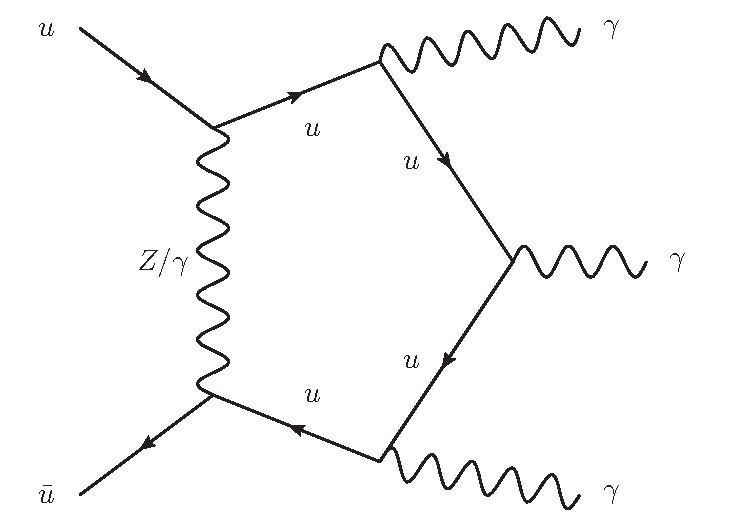
\includegraphics[width=0.288\textwidth]{diagrams/aaa_V_2} & &
    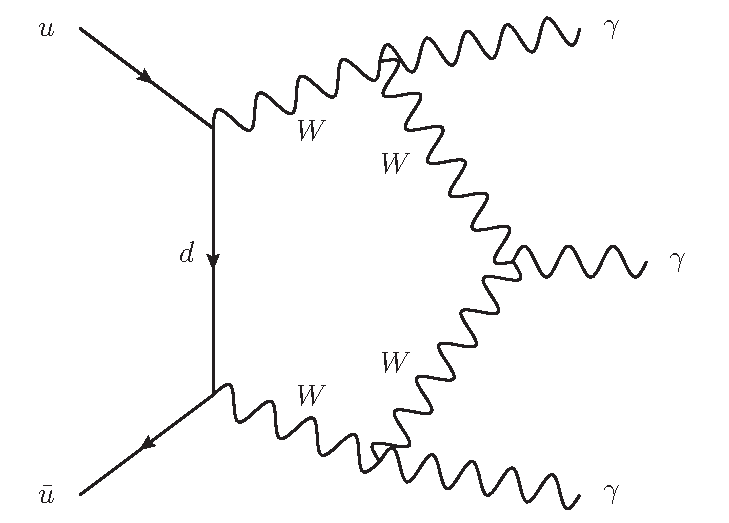
\includegraphics[width=0.288\textwidth]{diagrams/aaa_V_1} & &
    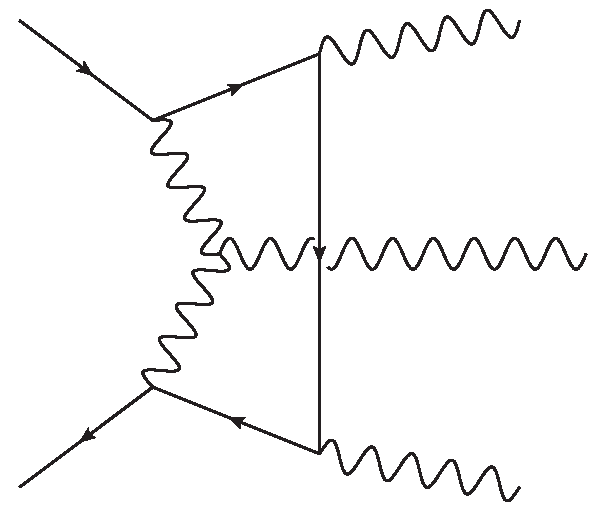
\includegraphics[width=0.288\textwidth]{diagrams/aaa_V_3} \\
  \end{tabular}
  \caption{
    Sample diagrams of electroweak virtual corrections to triple 
    photon production.
  }
\end{figure}

\begin{figure}[t!]
  \begin{tabular}{ccccc}
    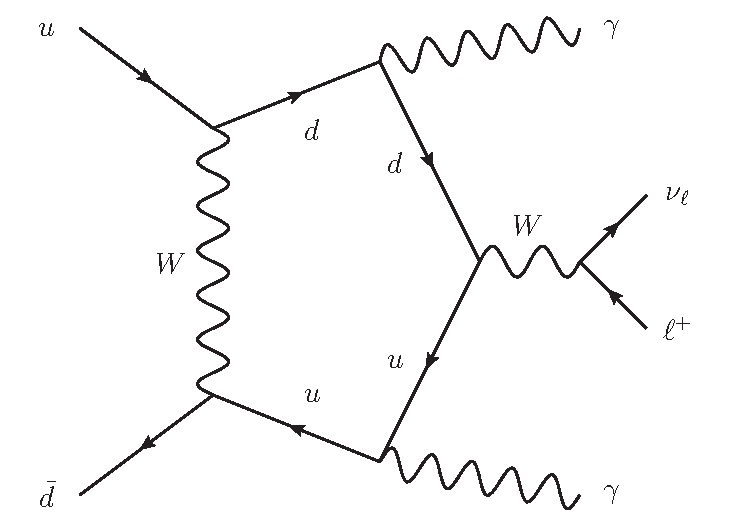
\includegraphics[width=0.288\textwidth]{diagrams/aaW_V_2} & &
    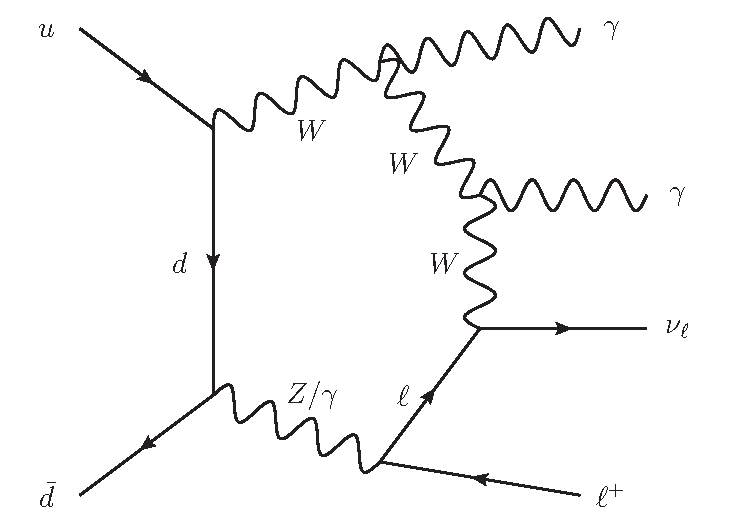
\includegraphics[width=0.288\textwidth]{diagrams/aaW_V_1} & &
    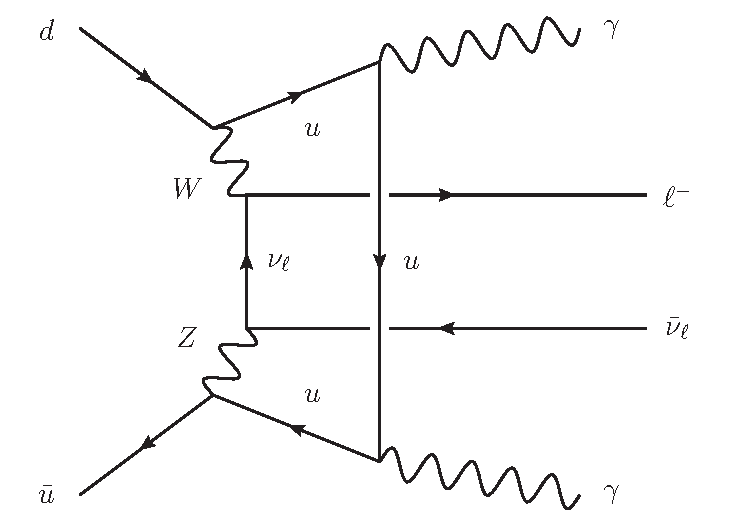
\includegraphics[width=0.288\textwidth]{diagrams/aaW_V_3} \\
  \end{tabular}
  \caption{
    Sample diagrams of electroweak virtual corrections to diphoton 
    production in association with a lepton-neutrino pair.
  }
\end{figure}

\begin{figure}[t!]
  \begin{tabular}{ccccc}
    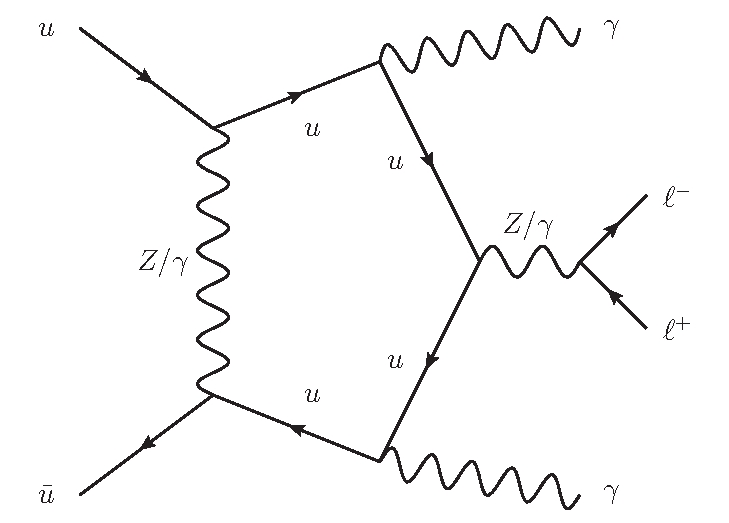
\includegraphics[width=0.288\textwidth]{diagrams/aaZ_V_2} & &
    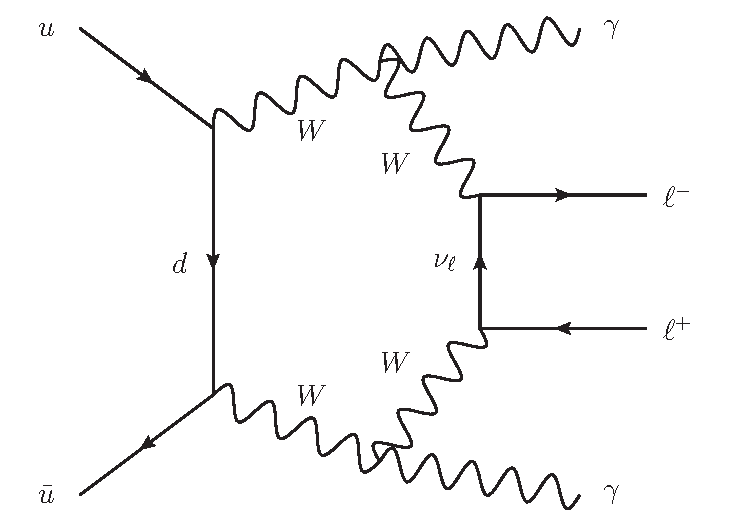
\includegraphics[width=0.288\textwidth]{diagrams/aaZ_V_1} & &
    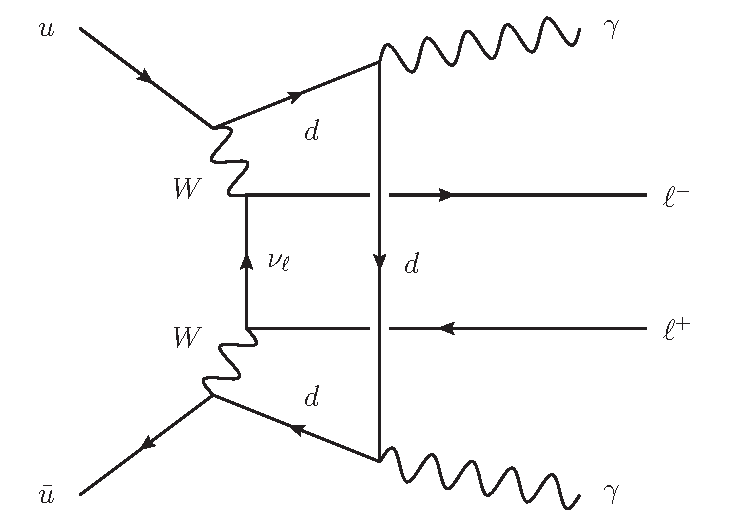
\includegraphics[width=0.288\textwidth]{diagrams/aaZ_V_3} \\
  \end{tabular}
  \caption{
    Sample diagrams of electroweak virtual corrections to diphoton 
    production in association with a lepton-pair.
  }
\end{figure}
